\section{Introduction}
\label{sec:intro}

Grammar rules apply not to individual words (e.g. dog, eat) but to
part-of-speech categories (e.g. noun, verb).  Thus learning
part-of-speech categories (also known as lexical or syntactic
categories) is one of the fundamental problems in language
acquisition.

Linguists identify part-of-speech categories based on semantic,
syntactic, and morphological properties of words.  There is also
evidence that children use prosodic and phonological features to
bootstrap part-of-speech category acquisition
\cite{ambridge2011child}.  However there is as yet no satisfactory
computational model that match human performance.  Thus identifying
the best set of features and best learning algorithms for
part-of-speech induction is still an open problem.

\begin{figure}[t] 
  \centering
  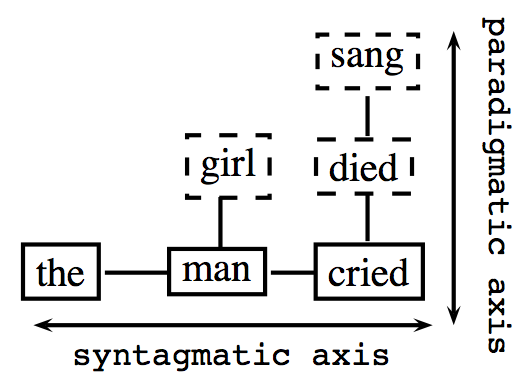
\includegraphics[height=0.3\textwidth]{paradigmatic.png}
  \caption{Syntagmatic vs. paradigmatic axes for words in a simple
    sentence \protect\cite{chandler2007semiotics}.}
  \label{fig:paradigmatic}
\end{figure}

Relationships between linguistic units can be classified into two
types: syntagmatic (concerning positioning), and paradigmatic
(concerning substitution).  Syntagmatic relations determine which
units can combine to create larger groups and paradigmatic relations
determine which units can be substituted for one another.
Figure~\ref{fig:paradigmatic} illustrates the paradigmatic vs
syntagmatic axes for words in a simple sentence and their possible
substitutes.  

Part-of-speech categories represent groups of words that can be
substituted for one another without altering the grammaticality of a
sentence.  In this paper we explore models of part-of-speech induction
based on potential substitutes of words.  We build {\em substitute
  word distributions} for each position in the text which specify the
probability of every vocabulary word in that position.
Table~\ref{tab:subdist} gives substitute distributions for an example
sentence.

\begin{table}[b]
\caption{The substitute word distributions (with probabilities in
  parentheses) for some of the positions in the example sentence
  \textit{``Pierre Vinken, 61 years old, will join the board as a
    nonexecutive director Nov.~29.''} based on an n-gram language
  model.}
\label{tab:subdist}
\begin{tabular}{|ll|} \hline
\textbf{will:} & \textit{will} (0.9985), \textit{would} (0.0007), \textit{to} (0.0006), \textit{also} (0.0001), $\ldots$ \\
\textbf{join:} & \textit{join} (0.6528), \textit{leave} (0.2140), \textit{oversee} (0.0559), \textit{head} (0.0262), \textit{rejoin} (0.0074), $\ldots$ \\
\textbf{the:}  &\textit{its} (0.9011), \textit{the} (0.0981), \textit{a} (0.0006), $\ldots$ \\
\textbf{board:} & \textit{board} (0.4288), \textit{company} (0.2584), \textit{firm} (0.2024), \textit{bank} (0.0731), \textit{strike} (0.0030), $\ldots$ \\
\hline
\end{tabular}
\end{table}

Note that the substitute word distribution for a position (e.g. the
second position in Fig.~\ref{fig:paradigmatic}) is a function of the
context only (i.e. \textit{``the \_\_\_ cried''}), and does not depend
on the word that actually appears there (i.e. ``man'').  Thus
substitute distributions represent {\em individual word contexts}, not
word types.  We refer to the use of features based on substitute
distributions as {\em paradigmatic representations of word context}.

We expect words used in similar contexts (with similar substitute
distributions) to share the same part-of-speech.  Thus part-of-speech
induction depends on which contexts are considered similar, and
context similarity in turn is a function of the features used to
represent word context.  Paradigmatic representations, using features
of the substitute distribution, uncover latent similarities between
contexts that on the surface seem to have little in common.  This
makes paradigmatic representations more robust to data sparsity,
compared to syntagmatic representations which use neighboring words as
features.  Our empirical results demonstrate that paradigmatic
representations significantly outperform syntagmatic ones when
compared using similar part-of-speech induction algorithms on
identical datasets.  Section~\ref{sec:representation} presents
alternative representations of word context and discusses paradigmatic
representations in more detail.

% talk about scode?
% talk about type vs token
% talk about the experiments

%% Part-of-speech induction can be performed on word types or word
%% tokens.  Induction on word types associates each word type with a
%% single category and cannot handle ambiguity: e.g. \textit{``join the
%%   board(n)''} vs. \textit{``board(v) the plane''}.


%% Our preliminary experiments on a subsection of 1M word Penn Treebank
%% Wall Street Journal corpus (PTB) \cite{treebank3} indicate that using
%% context information alone without the identity or the features of the
%% target word (e.g. using dimensionality reduction and clustering on
%% substitute vectors) has limited success and modeling the co-occurrence
%% of word and context types is essential for inducing syntactic
%% categories.  In order to do so, we combine paradigmatic
%% representations of word context with features of co-occurring words
%% within the co-occurrence data embedding (CODE) framework
%% \cite{globerson2007euclidean,maron2010sphere}.  The resulting
%% embeddings for word types are split into 45 clusters using k-means and
%% the clusters are compared to the 45 gold tags in the PTB.  We obtain
%% many-to-one accuracies up to .7680 using only distributional
%% information (the identity of the word and a representation of its
%% context) and .8023 by adding morphological and orthographic features
%% of the words improving the state-of-the-art in unsupervised part of
%% speech induction performance on the PTB.  We extend the experiments to
%% 19 corpora in 15 languages and achieve state-of-the-art many-to-one
%% (\mto) scores on 17 of them.

%% The next section gives a detailed review of related work.
%% Section~\ref{sec:subthr} describes the construction of the substitute
%% vectors and applies various distance metrics, dimensionality reduction
%% and clustering methods on substitute vectors of the PTB.
%% Section~\ref{sec:code} describes co-occurrence data embedding
%% (i.e. the learning algorithm used in our later experiments),
%% introduces possible usage scenarios of substitute vectors and
%% determines the best setup on the PTB.  Section~\ref{sec:multilang}
%% extends experiments to 15 languages and compares our results with the
%% best published results.  Section~\ref{sec:discuss} gives a brief error
%% analysis and Section~\ref{sec:contrib} summarizes our contributions.
%% All the data and the code to replicate the results given in this paper
%% is available from the authors' website at \mbox{\url{xxx.xxx.xxx}}.

%% Computational models of syntactic category acquisition rely mainly on
%% distributional analysis: Words that share the same distribution
%% (i.e. that occur in the same context) are grouped into the same
%% category.  The definition of ``the same context'' vary across studies.
%% Algorithms based on the Hidden Markov Model use class based n-grams to
%% specify context \cite{Brown:1992:CNG:176313.176316}, others use a
%% frame of neighboring words around the target word
%% \cite{Schutze:1995:DPT:976973.976994}.

%% Our hypothesis is that potential substitutes of a word are directly
%% indicative of its syntactic category and should be useful in acquiring
%% syntactic categories in general.  

%% Our main contribution in this study
%% is to introduce paradigmatic features, i.e. features based on
%% potential substitutes of the target word, to represent word context.

%% Both syntagmatic and paradigmatic relations of a word can be used to
%% represent its context.  In the syntagmatic case the context is
%% represented by a selection of neighboring words, in the paradigmatic
%% case it is represented by a set of possible substitutes.  In previous
%% studies of syntactic category learning the context representation has
%% been primarily syntagmatic, either implicit in the class based n-grams
%% of the standard Hidden Markov Model, or explicit in the construction
%% and clustering of left and right neighbors.

%% In this study we explore a paradigmatic representation of the context
%% of a word in syntactic category acquisition.  Specifically, the
%% context of a word is represented by a list of its possible substitutes
%% and their probabilities, which we call the {\em substitute vector}.
%% Note that the substitute vector is a function of the context only, not
%% the target word.  Thus in effect we are clustering contexts, not
%% words.  When word contexts are clustered based on their substitute
%% vectors they reveal a grouping that largely match the traditional part
%% of speech boundaries (\bestResult many-to-one score using a
%% 45-tag 24K word test corpus).
%% % standard HMM-EM gives 42\% on the same data.

%% Section~\ref{sec:related} gives a detailed review of related work.
%% The construction of the substitute vectors is described in
%% Section~\ref{sec:lm}.  To find out how to best make use of this new
%% paradigmatic representation, we explore different distance metrics
%% (Section~\ref{sec:dist}), dimensionality reduction methods
%% (Section~\ref{sec:dimreduce}), and clustering algorithms
%% (Section~\ref{sec:clustering}) for substitute vectors.  We note that
%% close to 95\% of the word occurrences in human labeled data are tagged
%% with their most frequent part of speech
%% \cite{Lee:2010:STU:1870658.1870741}, making one-tag-per-word a fairly
%% good first approximation.  Even ambicategory words generally have
%% fairly skewed part of speech distributions.
%% Section~\ref{sec:sparsity} looks at ways to increase the sparsity of
%% our solutions and demonstrates significant improvements using the
%% one-tag-per-word assumption and similarity metrics that introduce
%% sparsity.  Section~\ref{sec:discussion} discusses the results and
%% Section~\ref{sec:contrib} summarizes our contributions.

